%% This Beamer template is based on the one found here: https://github.com/sanhacheong/stanford-beamer-presentation, and edited to be used for Stanford ARM Lab

\documentclass[10pt]{beamer}
%\mode<presentation>{}

\usepackage{media9}
\usepackage{amssymb,amsmath,amsthm,enumerate}
\usepackage{mathtools}
\usepackage[utf8]{inputenc}
\usepackage{array}
\usepackage[parfill]{parskip}
\usepackage[utf8]{vietnam}
\usepackage{graphicx,animate}
\usepackage{caption}
\usepackage{subcaption}
\usepackage{bm}
\usepackage{amsfonts,amscd}
\usepackage[]{units}
\usepackage{listings}
\usepackage{multicol}
\usepackage{multirow}
\usepackage{tcolorbox}
\usepackage{physics}
\usepackage{movie15}
% Enable colored hyperlinks
\hypersetup{colorlinks=true}

% The following three lines are for crossmarks & checkmarks
\usepackage{pifont}% http://ctan.org/pkg/pifont
\newcommand{\cmark}{\ding{51}}%
\newcommand{\xmark}{\ding{55}}%

% Numbered captions of tables, pictures, etc.
\setbeamertemplate{caption}[numbered]
\usepackage{media9} 
%\usepackage[superscript,biblabel]{cite}
%\usepackage{algorithmic}
%\usepackage{algorithm2e}
%\usepackage{algpseudocode}
\usepackage[linesnumbered,ruled,vlined]{algorithm2e}
%\usepackage{algorithm}
%\usepackage{algorithmic}
\usepackage{caption}
%\usepackage{xcolor}
\usepackage{array}
%\renewcommand{\thealgocf}{}

\usepackage[natbib,backend=biber,style=ieee, sorting=ynt]{biblatex}
\bibliography{ref.bib}

\usepackage[acronym]{glossaries}

\usepackage{graphicx}
\graphicspath{{./figures}}
\usepackage{hyperref}

\usepackage{adjustbox}
\usepackage{fancyvrb}

\theoremstyle{remark}
\newtheorem*{remark}{Remark}
\theoremstyle{definition}

%\newcommand{\empy}[1]{{\color{darkorange}\emph{#1}}}
%\newcommand{\empr}[1]{{\color{cardinalred}\emph{#1}}}
%\newcommand{\examplebox}[2]{
%\begin{tcolorbox}[colframe=darkcardinal,colback=boxgray,title=#1]
%#2
%\end{tcolorbox}}

%\usetheme{Stanford} 
%\input{./style_files_stanford/my_beamer_defs.sty}
\usetheme{Copenhagen}
\usecolortheme{seahorse}
\logo{
\includegraphics[height=0.5in]{logos/HUS-name.jpg}}

\makeatletter
\let\@@magyar@captionfix\relax
\makeatother

\title[Phân tích dữ liệu cuộc bầu cử Tổng thống Mỹ năm 2020]{Phân tích dữ liệu cuộc bầu cử \\ Tổng thống Mỹ năm 2020}

\AtBeginSection[]
{
    \begin{frame}
        \frametitle{Nội dung}
        \tableofcontents[currentsection, subsectionstyle=show/show/hide]
    \end{frame}
}

\setbeamertemplate{page number in head/foot}[totalframenumber]
\setbeamertemplate{frametitle continuation}{}

\begin{document}
\nocite{*}

\author[Nguyễn Chí Thanh - 21007925]{
	\begin{tabular}{c} 
	\Large
	Nguyễn Chí Thanh \\
    \footnotesize \href{mailto:nguyenchithanh\_sdh21@hus.edu.vn}{nguyenchithanh\_sdh21@hus.edu.vn}
\end{tabular}
\vspace{-4ex}}

\institute{
	\vskip 5pt
	\begin{figure}
		\centering
		\begin{subfigure}[t]{0.5\textwidth}
			\centering
			
\includegraphics[height=0.75in]{logos/HUS-logo.jpg}
		\end{subfigure}%
		~ 
		\begin{subfigure}[t]{0.5\textwidth}
			\centering
			
\includegraphics[height=0.75in]{logos/MIM-logo.png}
		\end{subfigure}
	\end{figure}
	\vskip 5pt	
	Đại học Quốc Gia Hà Nội \\
	Trường đại học Khoa học tự nhiên\\
	Khoa Toán - Cơ - Tin học
	\vskip 3pt
}

%\begin{noheadline}
\begin{frame}[plain] \maketitle \end{frame}
%\end{noheadline}
    
\setbeamertemplate{itemize items}[default]
\setbeamertemplate{itemize subitem}[circle]

\begin{frame}[plain]{Nội dung}
    \tableofcontents[hidesubsections]
\end{frame}

\section{Tổng quan về dữ liệu cuộc bầu cử}

\begin{frame}{Dữ liệu sử dụng}
    \begin{itemize}
        \item Dữ liệu bầu cử tại từng hạt: \url{https://www.kaggle.com/datasets/unanimad/us-election-2020}
        \item Dữ liệu nhân khẩu học tại từng hạt (năm 2017): \url{https://www.kaggle.com/datasets/muonneutrino/us-census-demographic-data}
        \item Dữ liệu GDP tại từng hạt (từ năm 2001 đến năm 2018): \url{https://www.kaggle.com/datasets/anasmahmood000/highest-gdp-counties-in-usa}
    \end{itemize}
\end{frame}


\begin{frame}{Dữ liệu bầu cử tại từng hạt}
	\begin{figure}[h!]
        \centering
        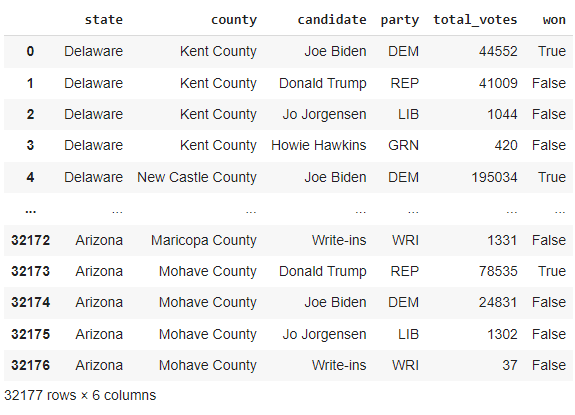
\includegraphics[width=0.8\textwidth]{figures/President_Dataframe.png}
        \caption{Dữ liệu về cuộc bầu cử tổng thống năm 2020 tại từng hạt}
    \end{figure}
\end{frame}

\begin{frame}{Dữ liệu bầu cử tại từng hạt}
	\begin{figure}[h!]
        \centering
        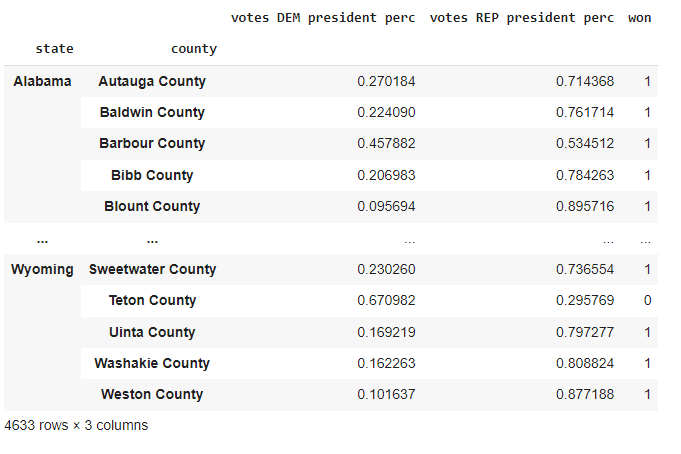
\includegraphics[width=0.8\textwidth]{figures/President_Dataframe_Rep_Dem_Percentage.png}
        \caption{Tỷ lệ phiếu bầu của các ứng cử viên tại từng hạt}
    \end{figure}
\end{frame}

\begin{frame}{Dữ liệu nhân khẩu học tại từng hạt}
	\begin{figure}[h!]
        \centering
        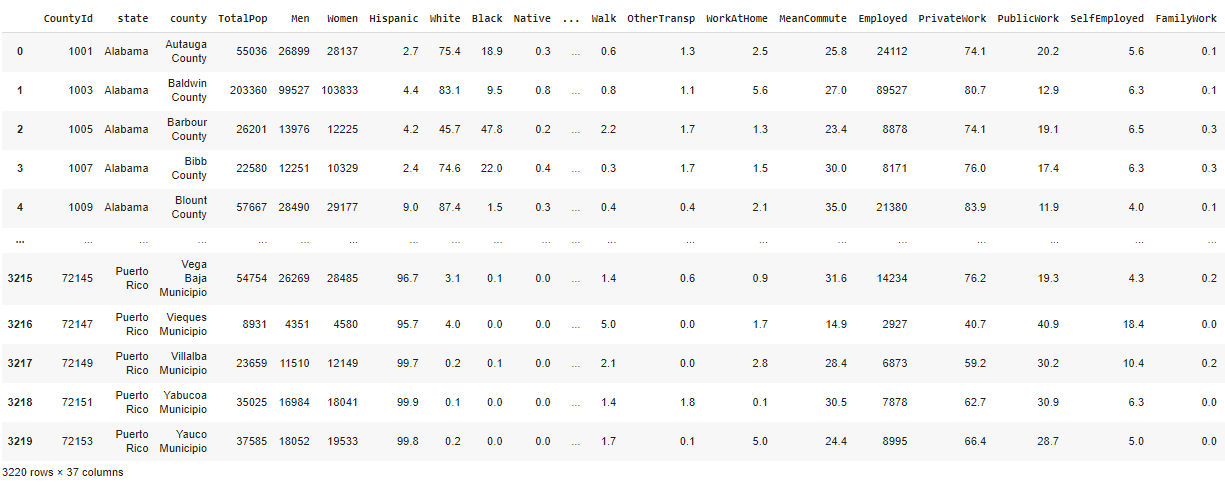
\includegraphics[width=\textwidth]{figures/Census_Dataframe.png}
        \caption{Dữ liệu về nhân khẩu học được hoàn thành vào năm 2017}
    \end{figure}
\end{frame}

\begin{frame}{Dữ liệu nhân khẩu học tại từng hạt}
	Ta chuẩn hóa dữ liệu nhân khẩu học bằng min-max scaling, sau đó ta sẽ kết hợp bảng dữ liệu phiếu bầu và bảng các yếu tố nhân khẩu học:
    \begin{figure}[h!]
        \centering
        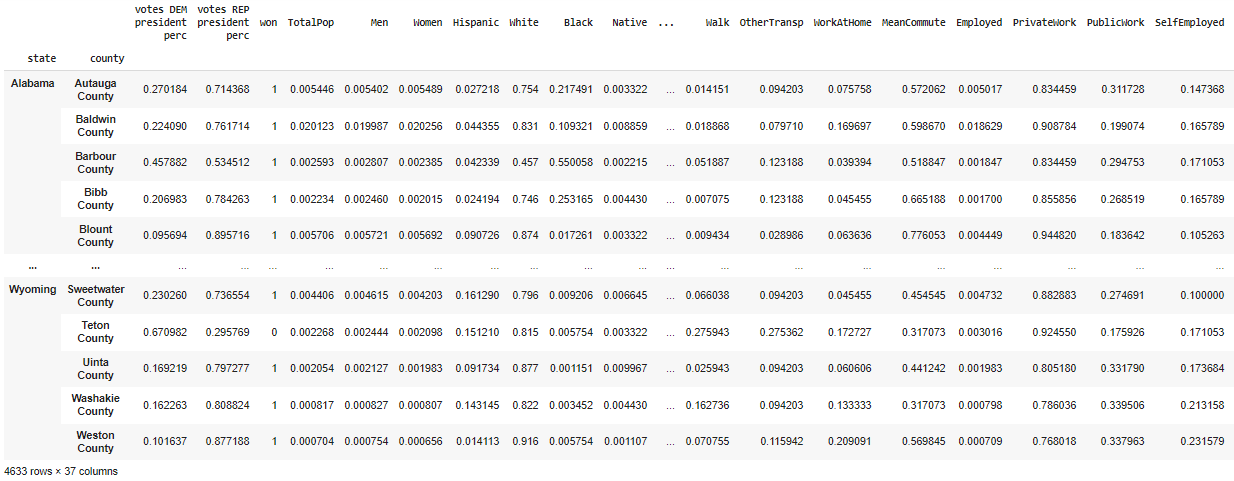
\includegraphics[width=\textwidth]{figures/President_Normalized_Demographic_Merged_Dataframe.png}
        \caption{Kết hợp bảng dữ liệu phiếu bầu và các yếu tố nhân khẩu học}
    \end{figure}
\end{frame}

\begin{frame}{Công cụ sử dụng}
    \begin{itemize}
        \item Trực quan hóa: Tableau trực quan hóa dữ liệu địa lý
        \item Phân tích độ quan trọng các đặc trưng: Mô hình hồi quy tuyến tính, XGBoost, Logistic Regression, Decision Tree, Random Forest,...
    \end{itemize}
\end{frame}

\section{Trực quan hóa dữ liệu kết quả cuộc bầu cử Tổng thống năm 2020}

\begin{frame}{Ứng cử viên Đảng Dân chủ}
    \begin{figure}[h!]
        \centering
        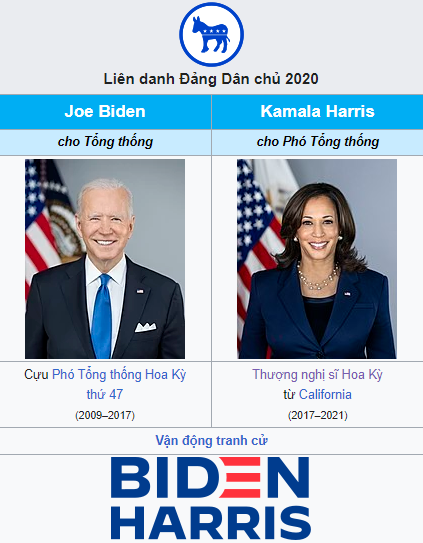
\includegraphics[height=0.8\textheight]{figures/Dem_Candidates.png}
        \caption{Hai ứng cử viên Đảng Dân chủ}
    \end{figure}
\end{frame}

\begin{frame}{Ứng cử viên Đảng Cộng hòa}
    \begin{figure}[h!]
        \centering
        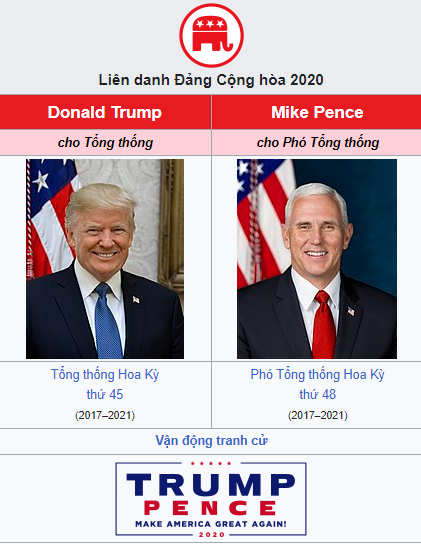
\includegraphics[height=0.8\textheight]{figures/Rep_Candidates.png}
        \caption{Hai ứng cử viên Đảng Cộng hòa}
    \end{figure}
\end{frame}

\begin{frame}{Ứng cử viên Đảng Tự do}
    \begin{figure}[h!]
        \centering
        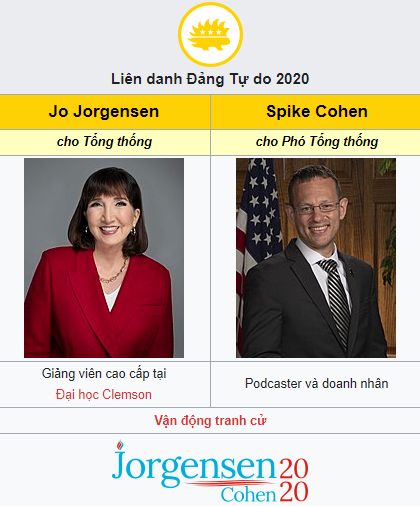
\includegraphics[height=0.8\textheight]{figures/Lib_Candidates.png}
        \caption{Hai ứng cử viên Đảng Tự do}
    \end{figure}
\end{frame}

\begin{frame}{Ứng cử viên Đảng Xanh}
    \begin{figure}[h!]
        \centering
        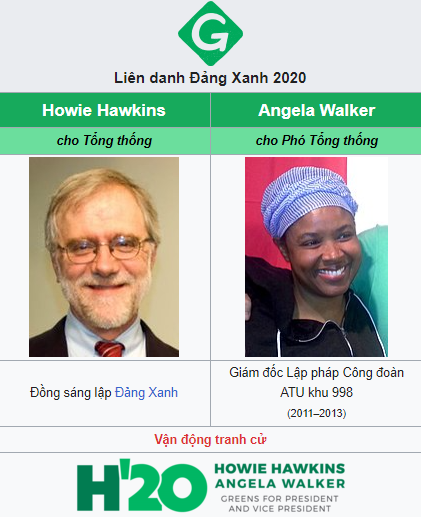
\includegraphics[height=0.8\textheight]{figures/Green_Candidates.png}
        \caption{Hai ứng cử viên Đảng Xanh}
    \end{figure}
\end{frame}

\begin{frame}{Số lá phiếu Đại cử tri theo từng bang}
	\begin{figure}[h!]
        \centering
        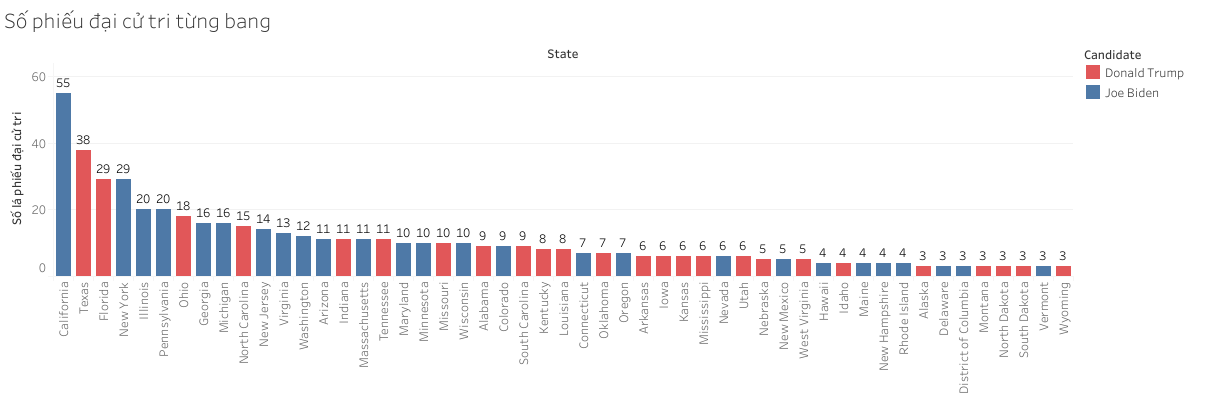
\includegraphics[width=\textwidth]{figures/State_Electoral_Votes_Bar_Chart.png}
        \caption{Tổng số phiếu Đại cử tri theo từng bang}
    \end{figure}
\end{frame}


\begin{frame}{Kết quả chung cuộc}
	\begin{figure}[h!]
        \centering
        \begin{subfigure}[b]{\textwidth}
            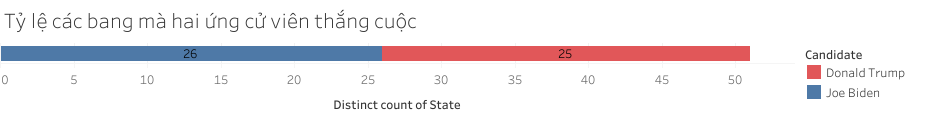
\includegraphics[width=0.9\textwidth]{figures/State_Candidate_Win.png}
            \caption{Số bang mà các ứng cử viên thắng}
        \end{subfigure}
        \vfill
        \begin{subfigure}[b]{\linewidth}
            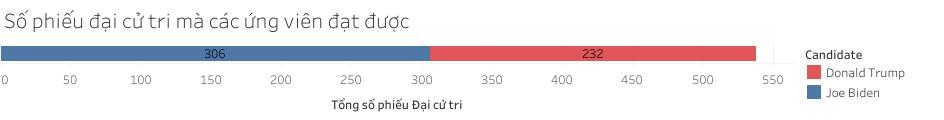
\includegraphics[width=0.9\linewidth]{figures/Electoral_Vote_Candidate_Win.png}
            \caption{Số phiếu Đại cử tri mà các ứng cử viên giành được}
        \end{subfigure}
        \caption{Kết quả chung cuộc của cuộc tranh cử Tổng thống Mỹ năm 2020}
    \end{figure}
\end{frame}

\begin{frame}{Kết quả chung cuộc}
	\begin{figure}[h!]
        \centering
        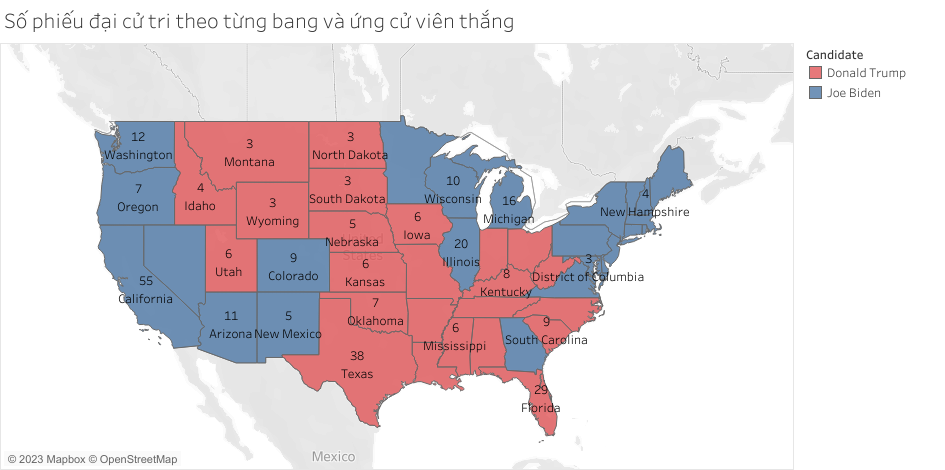
\includegraphics[width=\textwidth]{Electoral_Votes_States.png}
        \caption{Số phiếu đại cử tri theo từng bang và ứng cử viên thắng}
    \end{figure}
\end{frame}

\begin{frame}{Số lá phiếu phổ thông theo từng bang}
	\begin{figure}[h!]
        \centering
        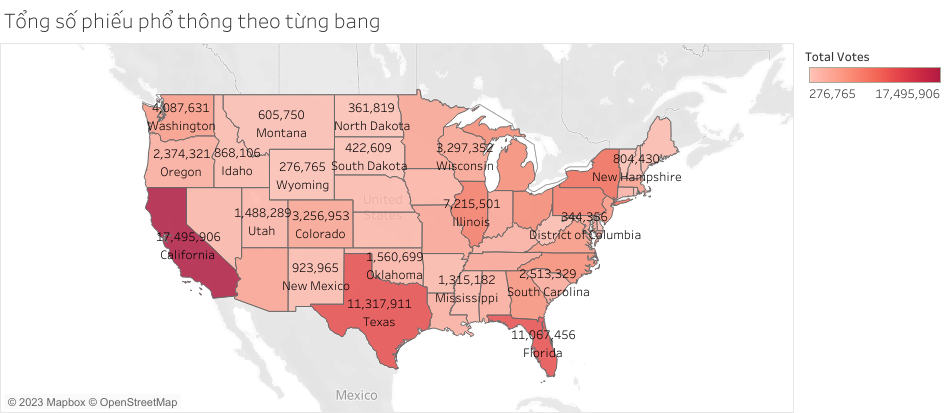
\includegraphics[width=\textwidth]{Popular_Votes_States_by_Color.png}
        \caption{Tổng số phiếu phổ thông theo từng bang}
    \end{figure}
\end{frame}

\begin{frame}{Bản đồ thể hiện tỷ lệ số lá phiếu phổ thông tại mỗi bang trên toàn liên bang}
	\begin{figure}[h!]
        \centering
        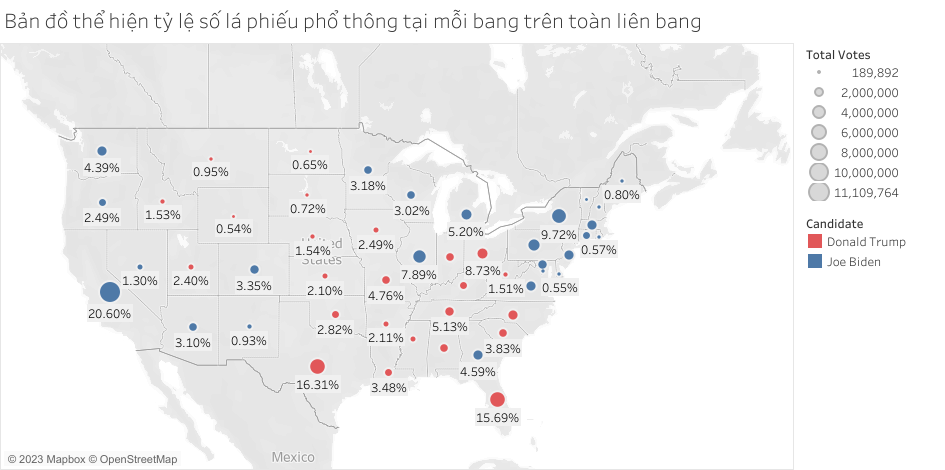
\includegraphics[width=\textwidth]{State_Percentage_Vote_Circle.png}
        \caption{Bản đồ thể hiện tỷ lệ số lá phiếu phổ thông tại mỗi bang trên toàn liên bang}
    \end{figure}
\end{frame}

\begin{frame}{Kết quả từng bang và tỷ lệ phiếu phổ thông từng ứng cử viên đạt được}
	\begin{figure}[h!]
        \centering
        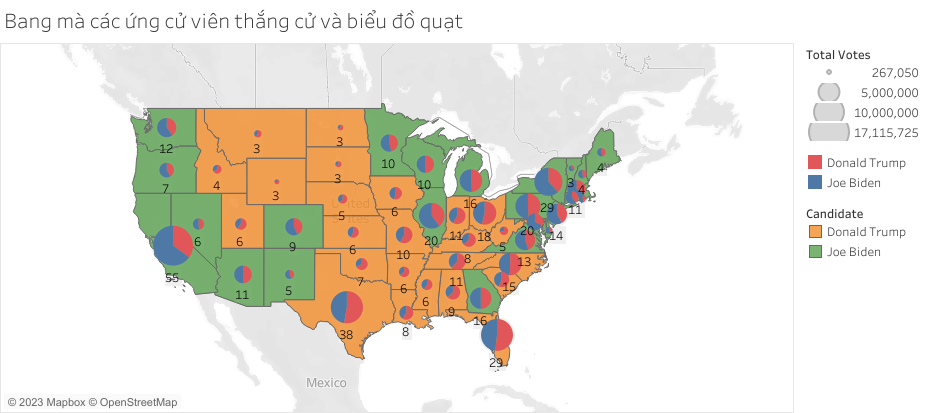
\includegraphics[width=\textwidth]{figures/State_Win_Candidate_and_Pie_chart.png}
        \caption{Kết quả từng bang và tỷ lệ phiếu phổ thông từng ứng cử viên đạt được}
    \end{figure}
\end{frame}

\begin{frame}{Tỷ lệ phiếu phổ thông của từng ứng viên}
	\begin{figure}[h!]
        \centering
        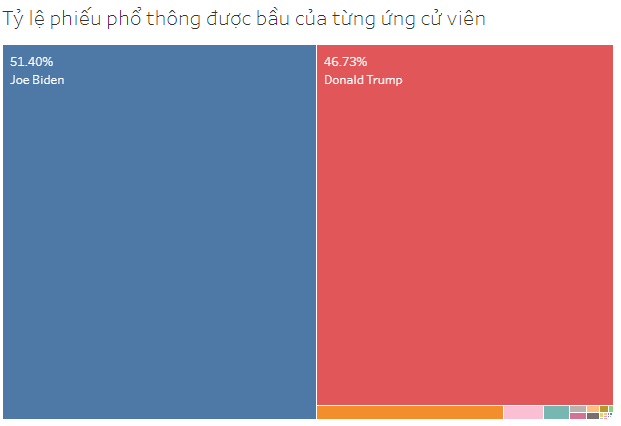
\includegraphics[width=0.6\textwidth]{Percentage_Total_Candidates_Tree_Chart.png}
        \caption{Tỷ lệ phiếu phổ thông được bầu của từng ứng cử viên}
    \end{figure}
\end{frame}

\begin{frame}{Tổng số phiếu phổ thông của từng ứng viên}
	\begin{figure}[h!]
        \centering
        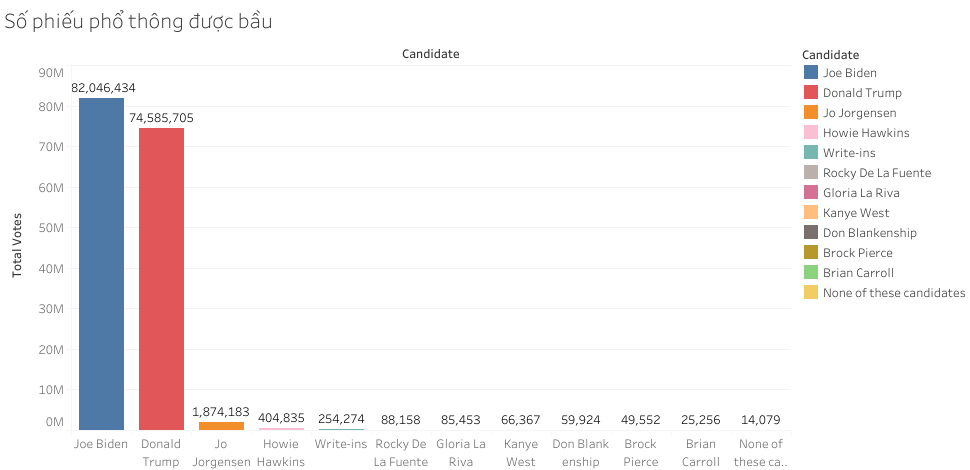
\includegraphics[width=\textwidth]{Total_Popular_Votes_Candidates_Bar_Chart.png}
        \caption{Tổng số phiếu phổ thông được bầu của từng ứng cử viên}
    \end{figure}
\end{frame}

\begin{frame}{Tỷ lệ số phiếu phổ thông của từng ứng viên tại từng bang}
	\begin{figure}[h!]
        \centering
        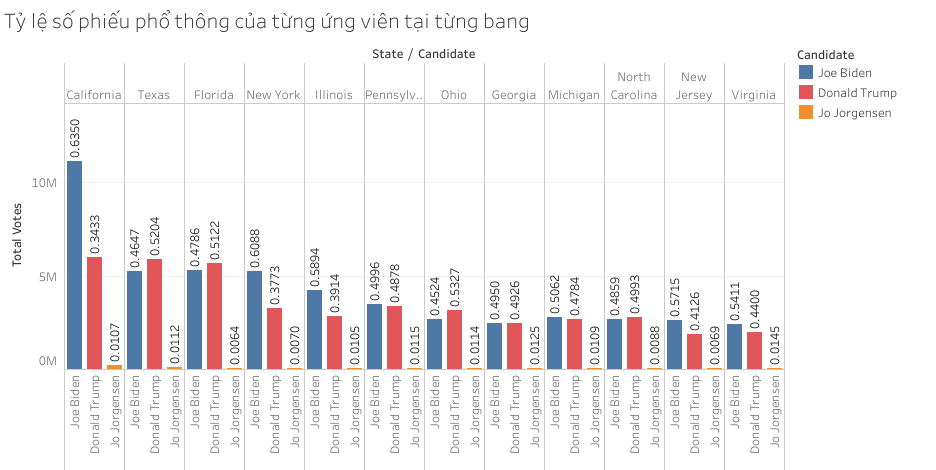
\includegraphics[width=\textwidth]{Percentage_Popular_Votes_Candidates_by_States.png}
        \caption{Tỷ lệ số phiếu phổ thông của từng ứng viên tại từng bang}
    \end{figure}
\end{frame}

\begin{frame}{Tỷ lệ số phiếu phổ thông của từng ứng viên tại từng bang}
	\begin{figure}[h!]
        \centering
        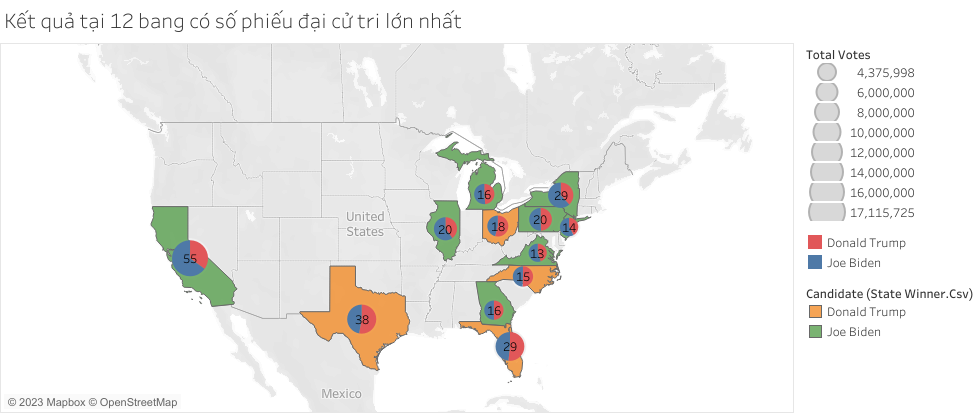
\includegraphics[width=\textwidth]{figures/12_Electoral_Vote_State_Candidate_Win.png}
        \caption{Tỷ lệ số phiếu phổ thông của từng ứng viên tại từng 12 bang có số phiếu Đại cử tri lớn nhất}
    \end{figure}
\end{frame}

\begin{frame}{Cartogram thể hiện tổng số lá phiếu phổ thông tương ứng với các ứng cử viên thắng cuộc}
	\begin{figure}[h!]
        \centering
        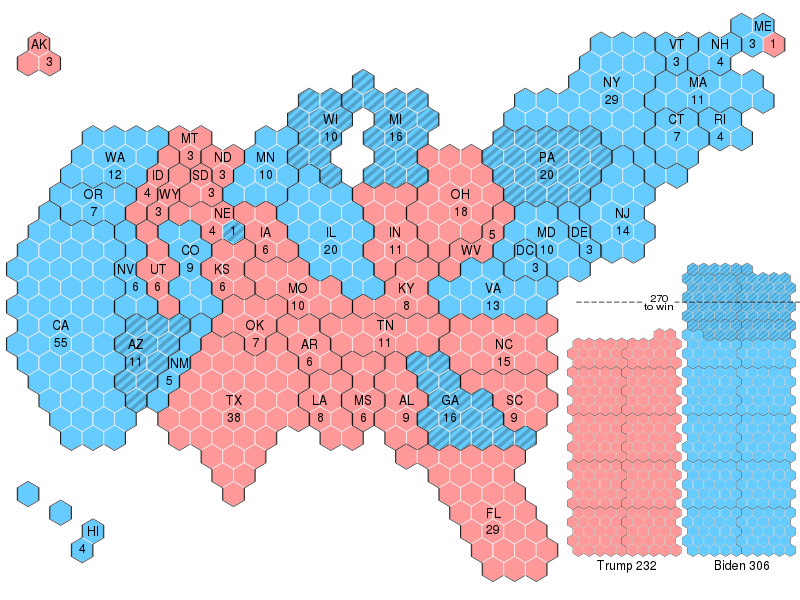
\includegraphics[width=0.7\textwidth]{State_Total_Vote_Cartogram.png}
        \caption{Cartogram thể hiện tổng số lá phiếu phổ thông tương ứng với các ứng cử viên thắng cuộc}
    \end{figure}
\end{frame}

\begin{frame}{Tỷ lệ GDP của tiểu bang trên toàn liên bang}
	\begin{figure}[h!]
        \centering
        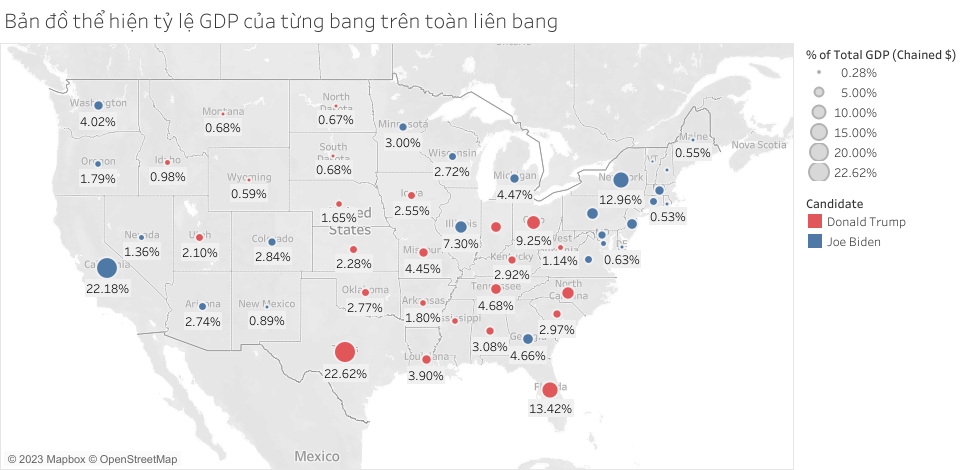
\includegraphics[width=\textwidth]{figures/State_Percentage_GDP_Circle.png}
        \caption{Tỷ lệ GDP của tiểu bang trên toàn liên bang}
    \end{figure}
\end{frame}

\begin{frame}{Kết quả bỏ phiếu tại các hạt}
	\begin{figure}[h!]
        \centering
        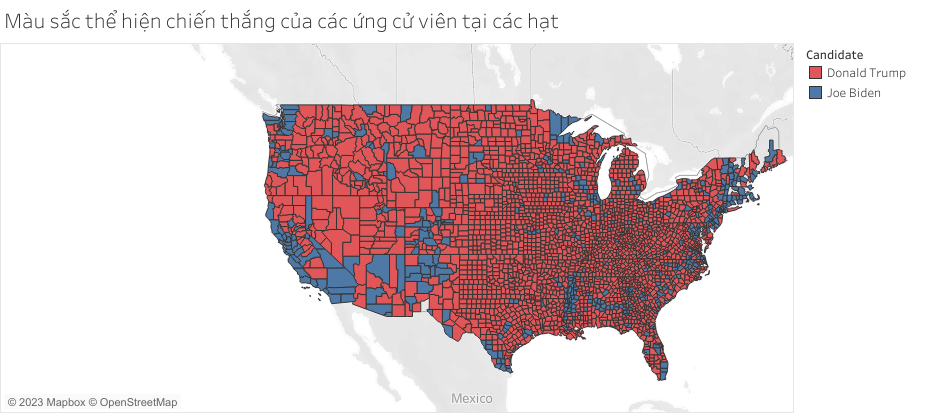
\includegraphics[width=0.9\textwidth]{County_Candidate_Win.png}
        \caption{Màu sắc thể hiện chiến thắng của các ứng cử viên tại các hạt}
    \end{figure}
\end{frame}

\begin{frame}{Tổng số lá phiếu phổ thông tại mỗi hạt}
	\begin{figure}[h!]
        \centering
        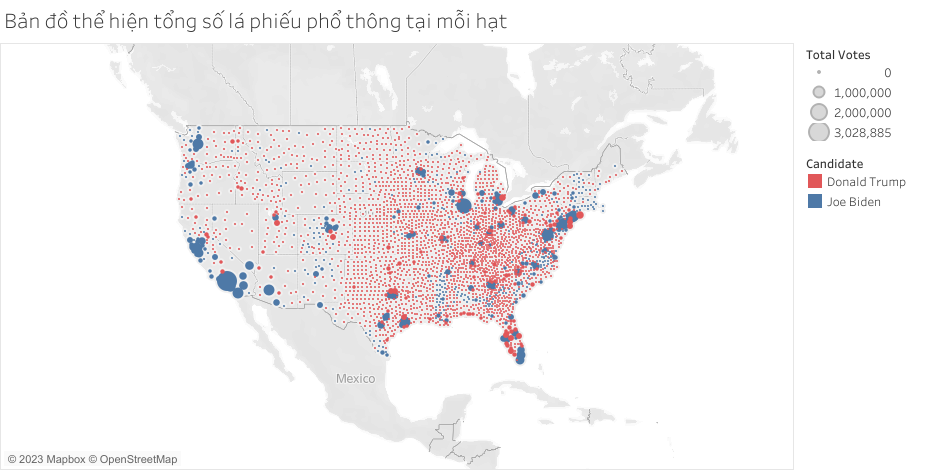
\includegraphics[width=\textwidth]{County_Total_Vote_Circle.png}
        \caption{Bản đồ thể hiện tổng số lá phiếu phổ thông tại mỗi hạt}
    \end{figure}
\end{frame}

\begin{frame}{Bản đồ thể hiện tổng dân số tại mỗi hạt}
	\begin{figure}[h!]
        \centering
        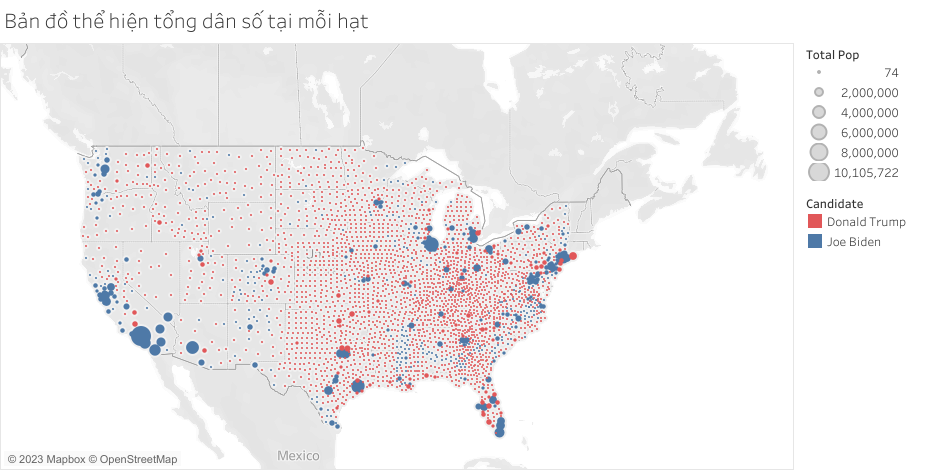
\includegraphics[width=0.9\textwidth]{figures/County_Total_Population_Circle.png}
        \caption{Bản đồ thể hiện tổng dân số tại mỗi hạt}
    \end{figure}
\end{frame}

\begin{frame}{So sánh quy mô dân số và kinh tế tại các bang, hạt mà các ứng cử viên chiến thắng}
	\begin{figure}[h!]
        \centering
        \begin{subfigure}[b]{\textwidth}
            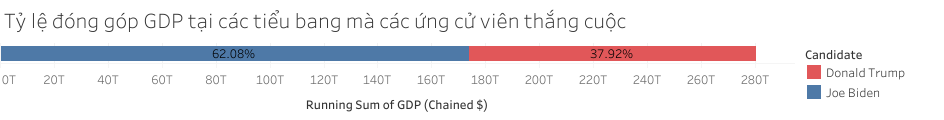
\includegraphics[width=0.9\textwidth]{State_Percentage_GDP_Candidate.png}
            \caption{Tỷ lệ đóng góp GDP tại các tiểu bang mà các ứng cử viên thắng}
        \end{subfigure}
        \vfill
        \begin{subfigure}[b]{\linewidth}
            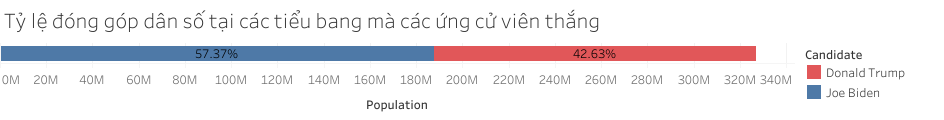
\includegraphics[width=0.9\linewidth]{State_Percentage_Population_Candidate.png}
            \caption{Tỷ lệ đóng góp dân số tại các tiểu bang mà các ứng cử viên thắng}
        \end{subfigure}
    \end{figure}
	
\end{frame}

\begin{frame}
    \begin{figure}[h!]
        \centering
        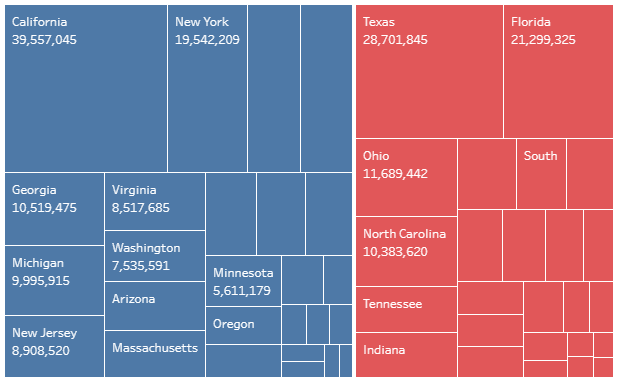
\includegraphics[width=0.9\textwidth]{figures/State_Population_Treemap.png}
        \caption{So sánh tổng dân số tại các bang mà các ứng cử viên chiến thắng}
    \end{figure}
\end{frame}

\begin{frame}
    \begin{figure}[h!]
        \centering
        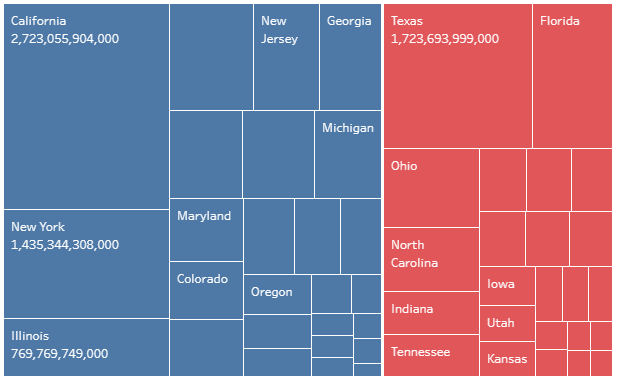
\includegraphics[width=0.9\textwidth]{figures/State_GDP_Treemap.png}
        \caption{So sánh tổng GDP tại các bang mà các ứng cử viên chiến thắng}
    \end{figure}
\end{frame}

\begin{frame}
	\begin{figure}[h!]
        \begin{subfigure}[b]{\textwidth}
            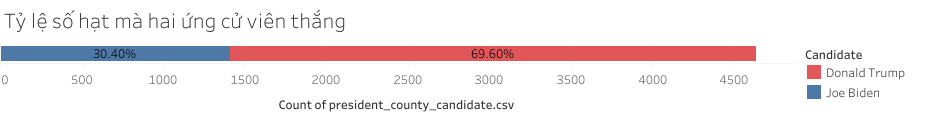
\includegraphics[width=0.9\linewidth]{County_Total_Percentage_Candidate_Win.png}
            \caption{Tỷ lệ thắng trên các hạt của từng ứng cử viên}
        \end{subfigure}
        \vfill
        \begin{subfigure}[b]{\textwidth}
            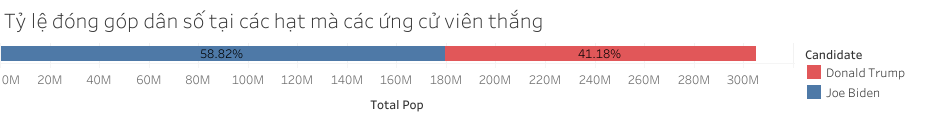
\includegraphics[width=0.9\linewidth]{County_Percentage_Population_Candidate.png}
            \caption{Tỷ lệ đóng góp dân số tại các hạt mà các ứng cử viên thắng}
        \end{subfigure}
    \end{figure}
\end{frame}

\begin{frame}
    \begin{figure}[h!]
        \centering
        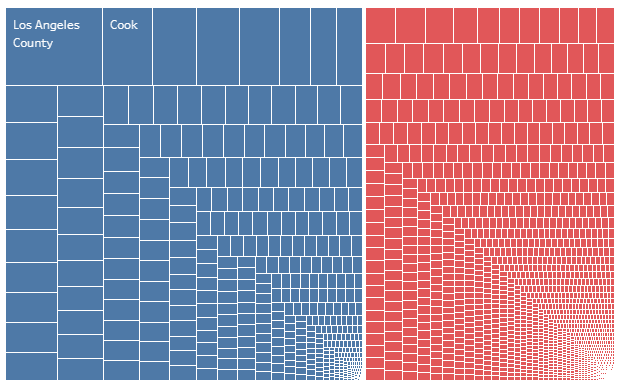
\includegraphics[width=0.9\textwidth]{figures/County_Population_Treemap.png}
        \caption{So sánh tổng dân số tại các hạt mà các ứng cử viên chiến thắng}
    \end{figure}
\end{frame}

\begin{frame}
    \begin{figure}[h!]
        \centering
        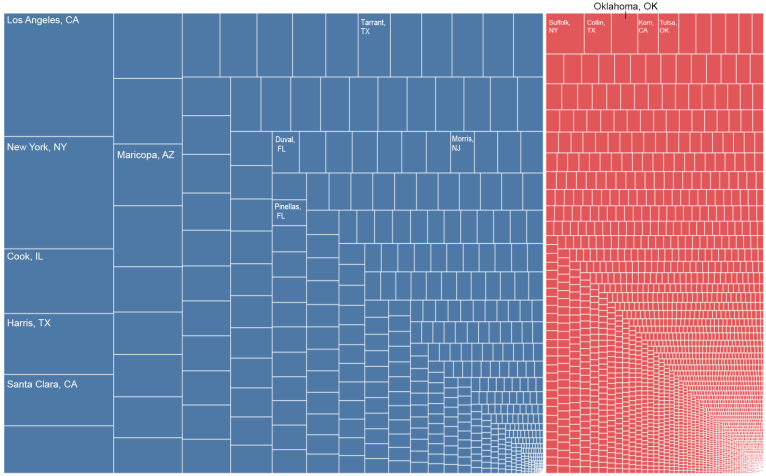
\includegraphics[width=0.9\textwidth]{figures/County_GDP_Treemap.png}
        \caption{So sánh tổng GDP tại các hạt mà các ứng cử viên chiến thắng}
    \end{figure}
\end{frame}

\begin{frame}
	\begin{figure}[h!]
        \centering
        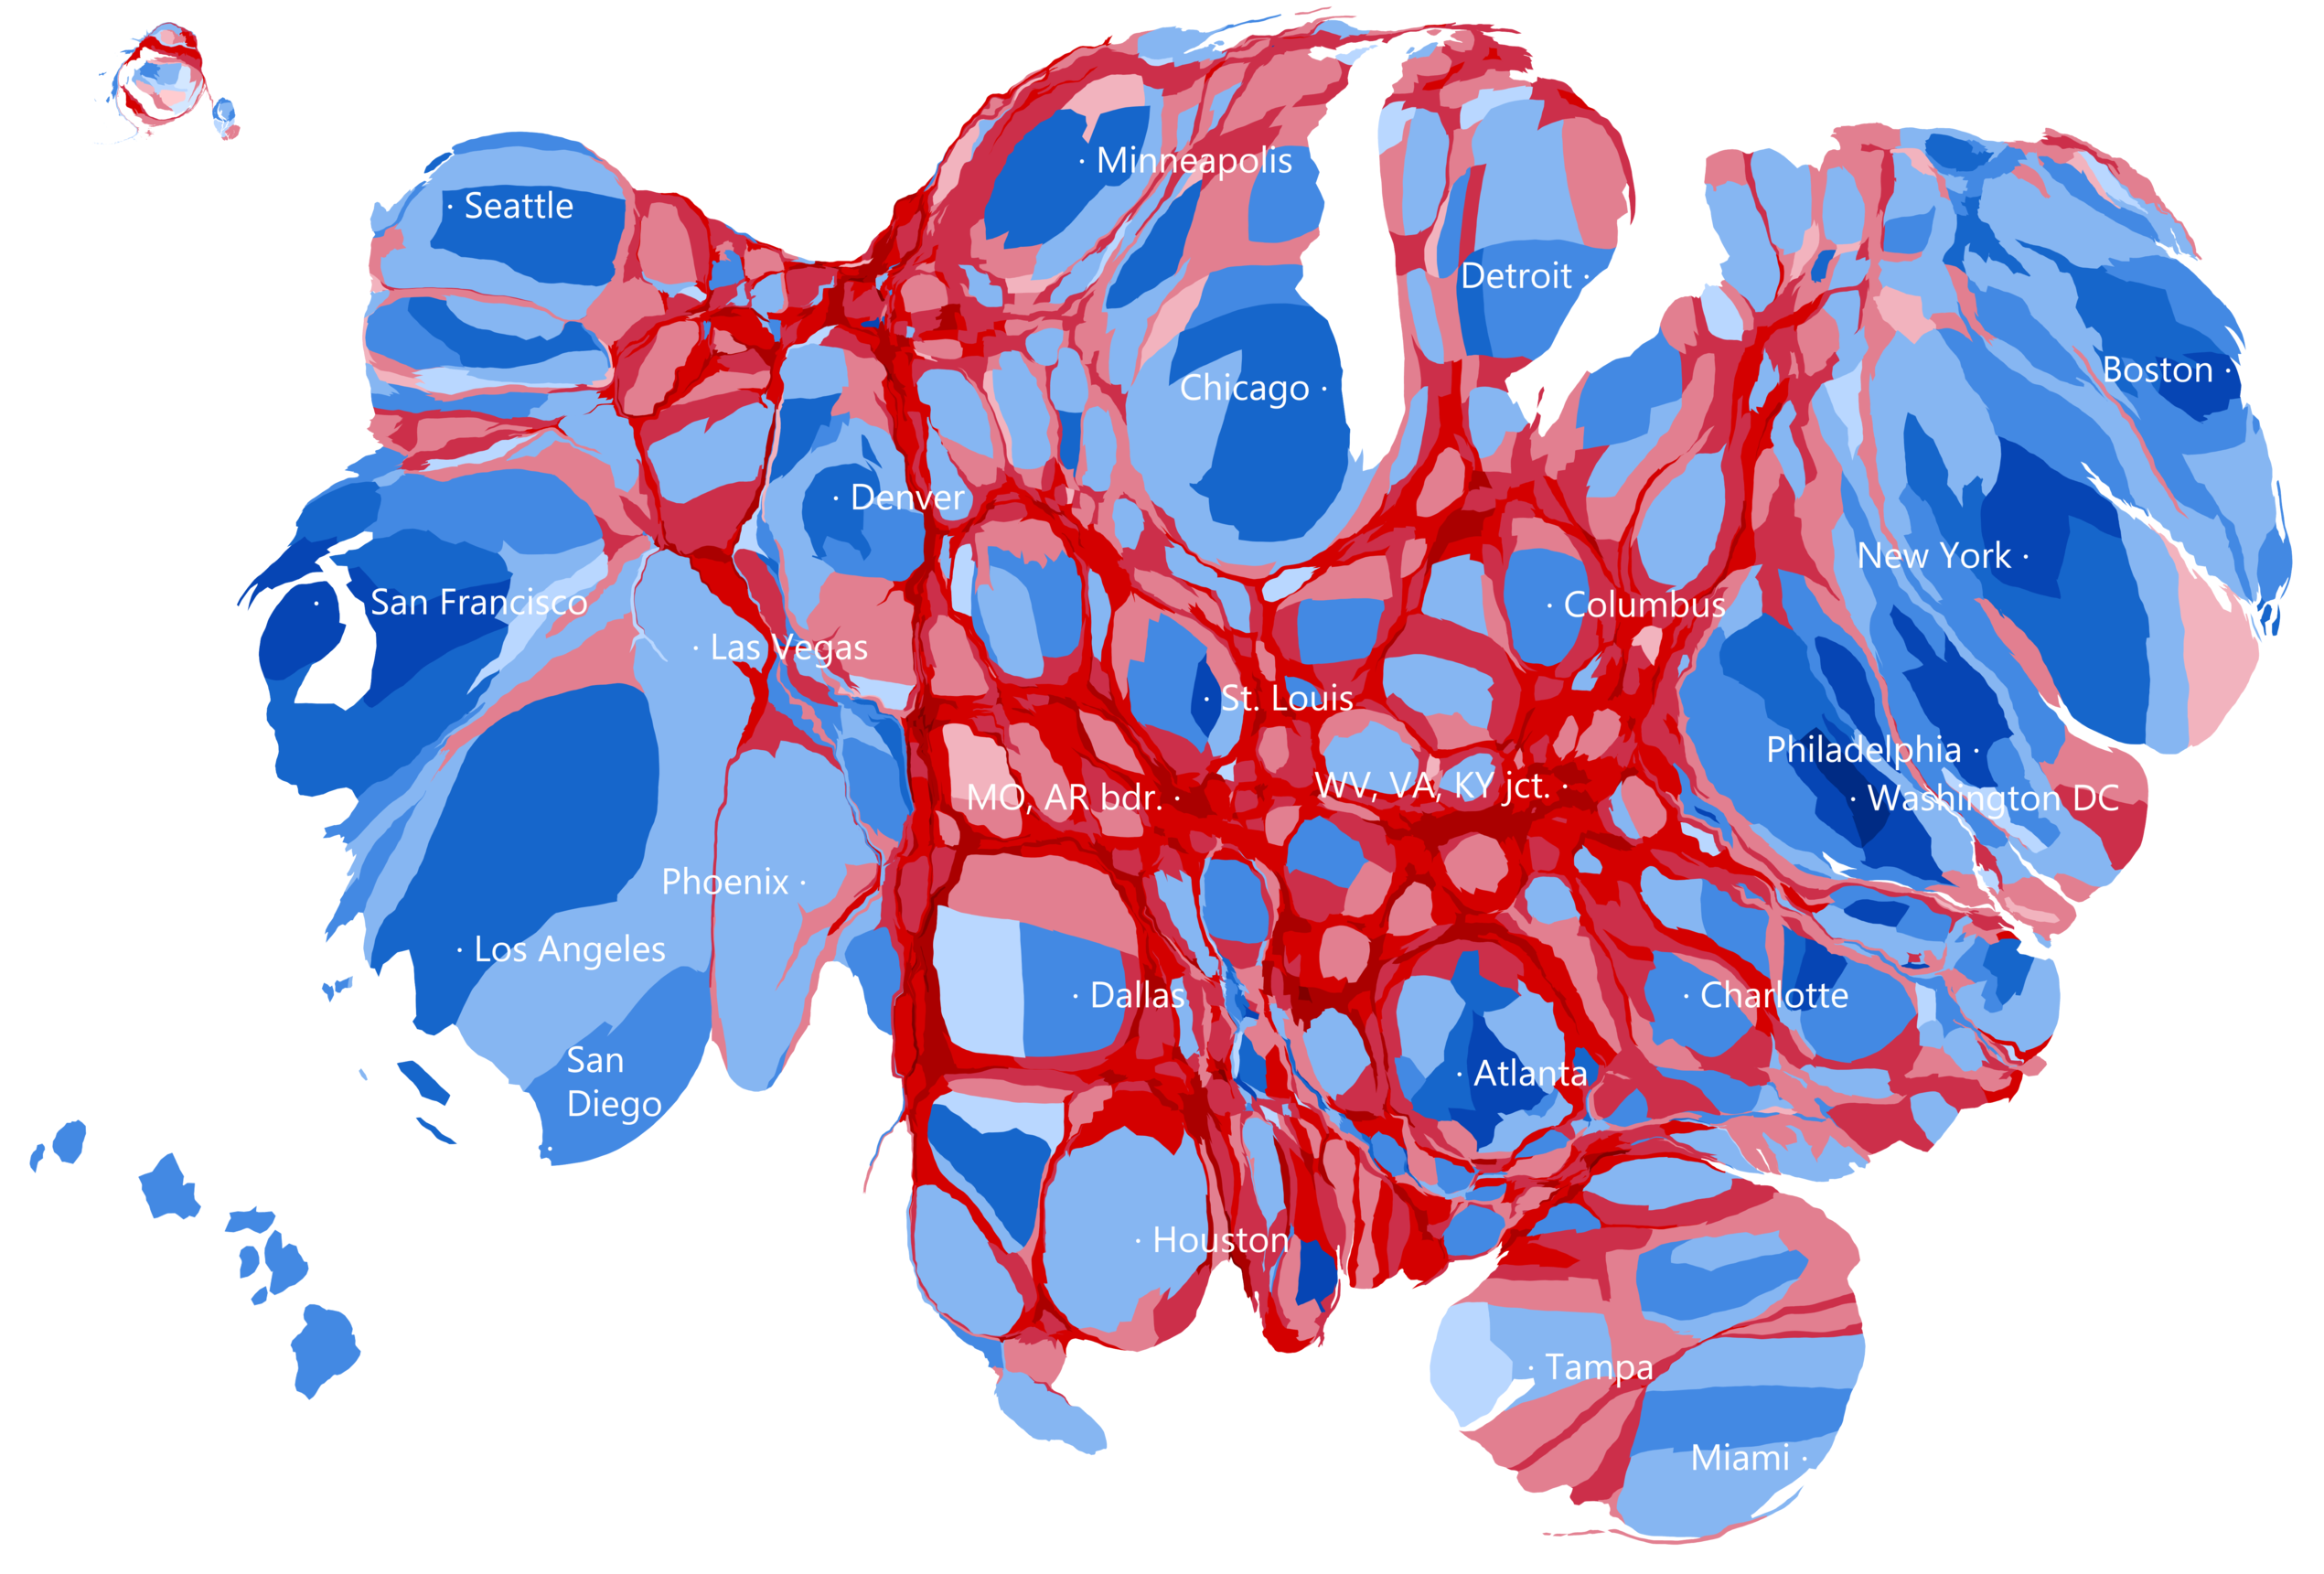
\includegraphics[width=0.9\textwidth]{figures/County_Total_Vote_Cartogram.png}
        \caption{Cartogram thể hiện tổng số lá phiếu phổ thông tương ứng với các ứng cử viên thắng cuộc trên cấp độ hạt}
    \end{figure}
\end{frame}

\begin{frame}{Khoảng cách tỷ lệ phiếu bầu giữa hai ứng cử viên tại các bang}
	\begin{figure}[h!]
        \centering
        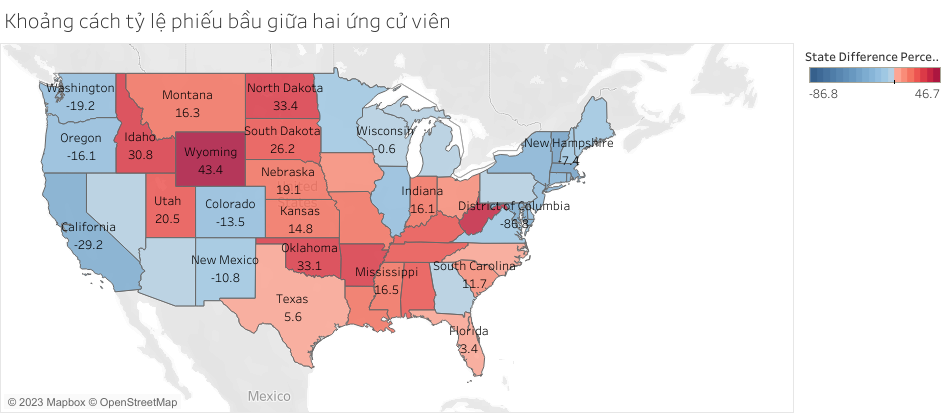
\includegraphics[width=\textwidth]{figures/State_Difference_Percentage_Total_Vote_Two_Candidate.png}
        \caption{Khoảng cách tỷ lệ phiếu bầu giữa hai ứng cử viên tại các bang}
    \end{figure}
\end{frame}

\begin{frame}{Khoảng cách tỷ lệ phiếu bầu giữa các ứng cử viên tại các hạt}
	\begin{figure}[h!]
        \centering
        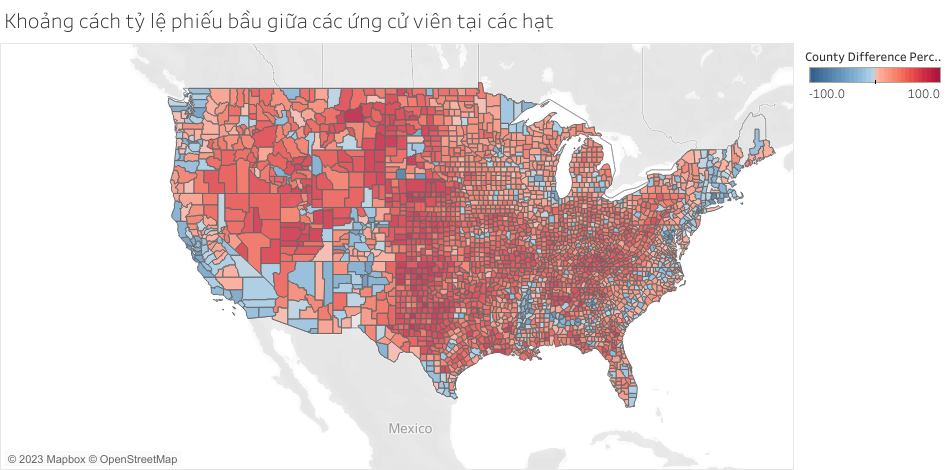
\includegraphics[width=\textwidth]{figures/County_Difference_Percentage_Total_Vote_Two_Candidate.png}
        \caption{Khoảng cách tỷ lệ phiếu bầu giữa các ứng cử viên tại các hạt}
    \end{figure}
\end{frame}



\begin{frame}{Biểu đồ cột thể hiện chênh lệch tỷ lệ phiếu bầu giữa các ứng viên trên từng tiểu bang}
	\begin{figure}[h!]
		\centering
		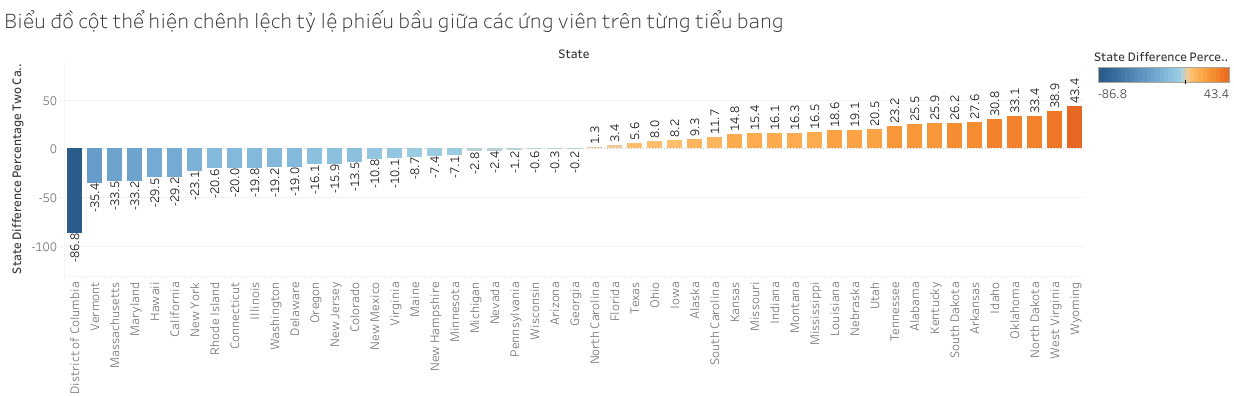
\includegraphics[width=0.9\textwidth]{figures/State_Difference_Percentage_Total_Vote_Two_Candidate_Bar_Chart.png}
		\caption{Biểu đồ cột thể hiện chênh lệch tỷ lệ phiếu bầu giữa các ứng viên trên từng tiểu bang}
	\end{figure}
\end{frame}


\begin{frame}{Tỷ lệ ủng hộ ứng cử viên theo quan điểm chính trị}
	\begin{figure}[h!]
        \centering
        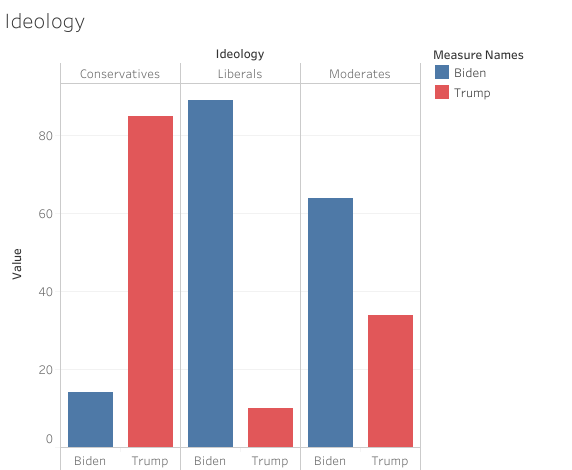
\includegraphics[width=0.7\textwidth]{figures/Ideology.png}
        \caption{Tỷ lệ ủng hộ ứng cử viên theo quan điểm chính trị}
    \end{figure}
\end{frame}


\begin{frame}{Tỷ lệ ủng hộ ứng cử viên theo đảng phái chính trị}
	\begin{figure}[h!]
        \centering
        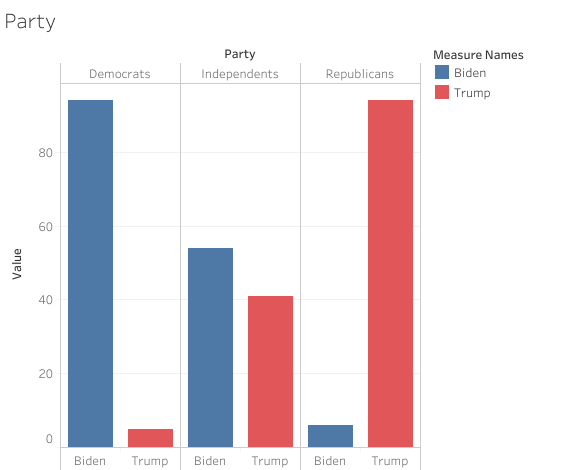
\includegraphics[width=0.7\textwidth]{figures/Party.png}
        \caption{Tỷ lệ ủng hộ ứng cử viên theo đảng phái chính trị}
    \end{figure}
\end{frame}


\begin{frame}{Tỷ lệ ủng hộ ứng cử viên theo tình trạng hôn nhân}
	\begin{figure}[h!]
        \centering
        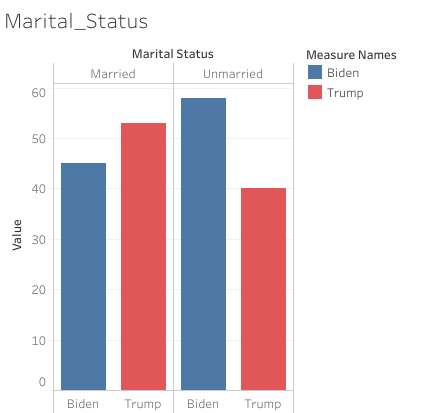
\includegraphics[width=0.6\textwidth]{figures/Marital_Status.png}
        \caption{Tỷ lệ ủng hộ ứng cử viên theo tình trạng hôn nhân}
    \end{figure}
\end{frame}


\begin{frame}{Tỷ lệ ủng hộ ứng cử viên theo giới tính và tình trạng hôn nhân}
	\begin{figure}[h!]
        \centering
        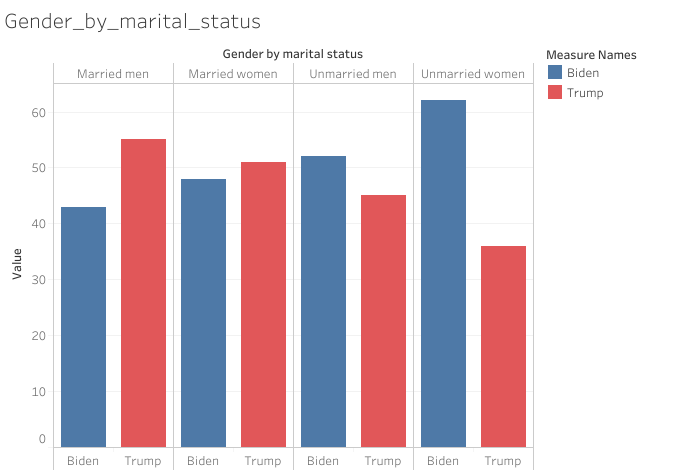
\includegraphics[width=0.7\textwidth]{figures/Gender_by_marital_status.png}
        \caption{Tỷ lệ ủng hộ ứng cử viên theo giới tính và tình trạng hôn nhân}
    \end{figure}
\end{frame}

\begin{frame}{Tỷ lệ ủng hộ ứng cử viên theo chủng tộc}
	\begin{figure}[h!]
        \centering
        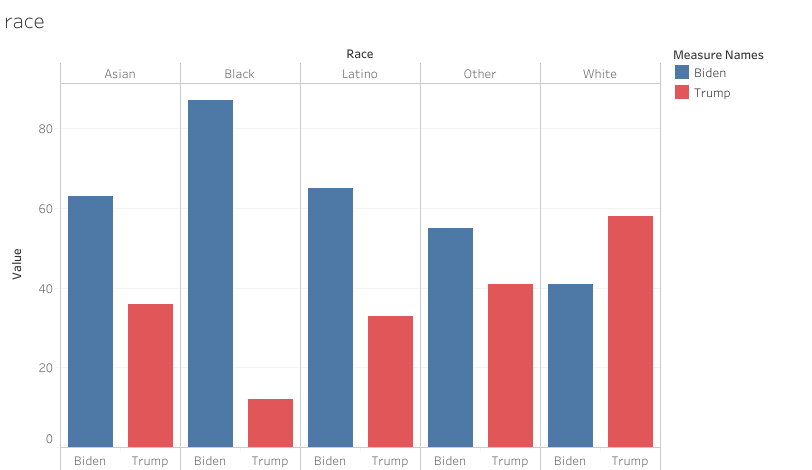
\includegraphics[width=0.7\textwidth]{figures/race.png}
        \caption{Tỷ lệ ủng hộ ứng cử viên theo chủng tộc}
    \end{figure}
\end{frame}

\begin{frame}{Tỷ lệ ủng hộ ứng cử viên theo giới tính và chủng tộc}
	\begin{figure}[h!]
        \centering
        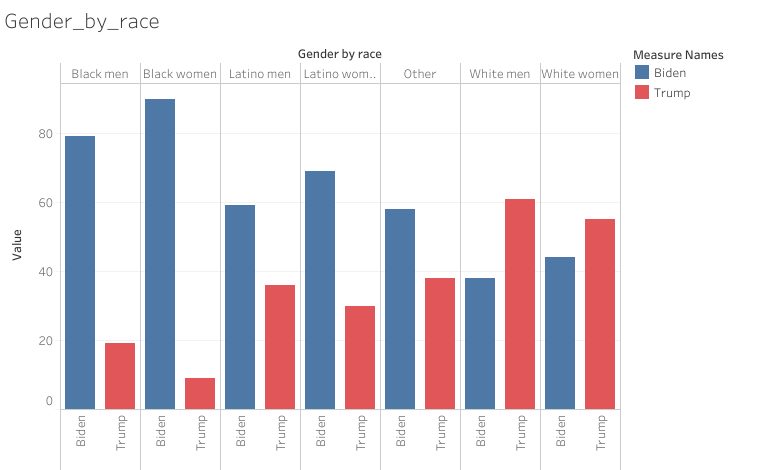
\includegraphics[width=0.7\textwidth]{figures/Gender_by_race.png}
        \caption{Tỷ lệ ủng hộ ứng cử viên theo giới tính và chủng tộc}
    \end{figure}
\end{frame}

\begin{frame}{Tỷ lệ ủng hộ ứng cử viên theo tôn giáo}
	\begin{figure}[h!]
        \centering
        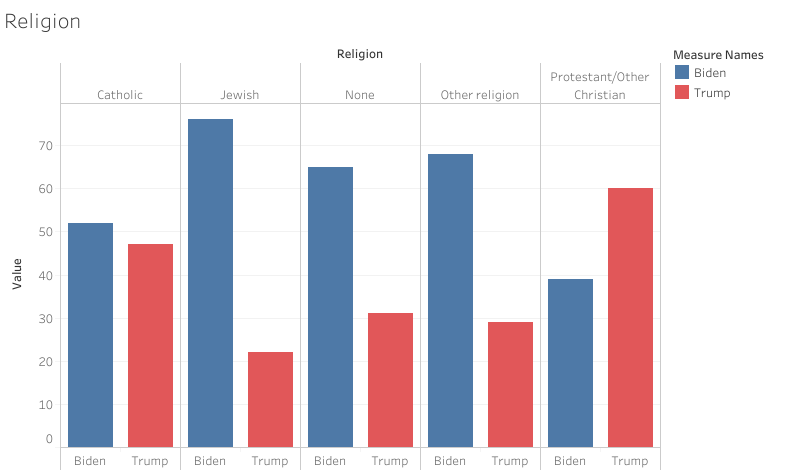
\includegraphics[width=0.7\textwidth]{figures/Religion.png}
        \caption{Tỷ lệ ủng hộ ứng cử viên theo tôn giáo}
    \end{figure}
\end{frame}

\begin{frame}{Tỷ lệ ủng hộ ứng cử viên theo độ tuổi}
	\begin{figure}[h!]
        \centering
        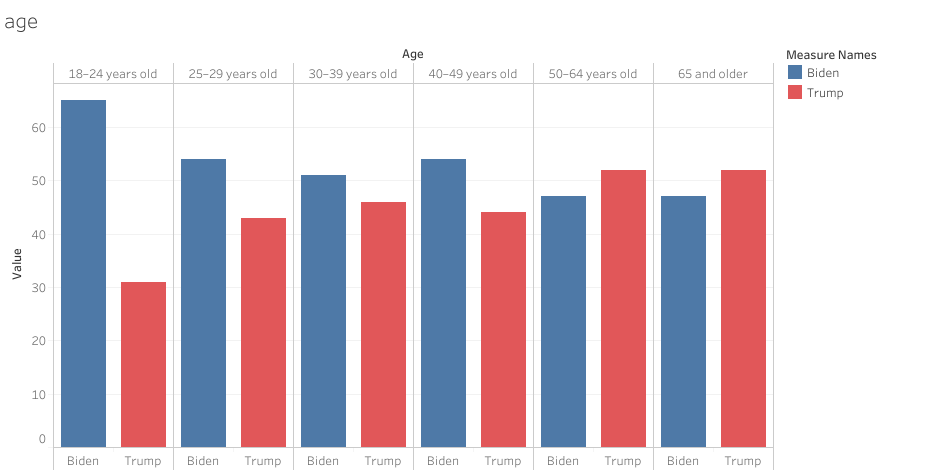
\includegraphics[width=0.7\textwidth]{figures/age.png}
        \caption{Tỷ lệ ủng hộ ứng cử viên theo độ tuổi}
    \end{figure}
\end{frame}


\begin{frame}{Tỷ lệ ủng hộ ứng cử viên theo độ tuổi và chủng tộc}
	\begin{figure}[h!]
        \centering
        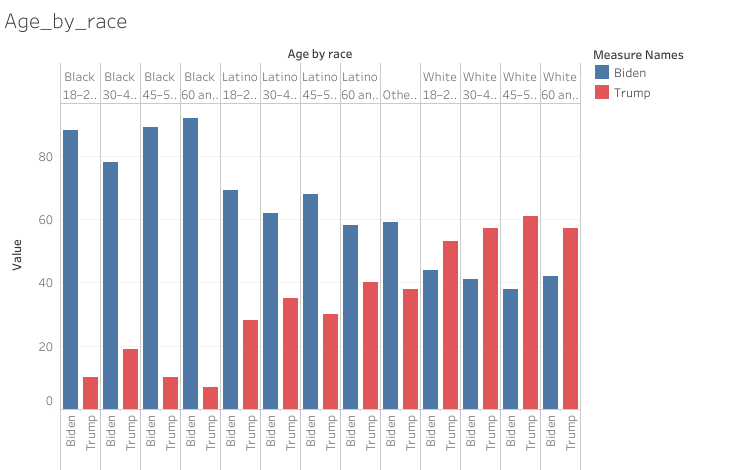
\includegraphics[width=0.8\textwidth]{figures/Age_by_race.png}
        \caption{Tỷ lệ ủng hộ ứng cử viên theo độ tuổi và chủng tộc}
    \end{figure}
\end{frame}

\begin{frame}{Tỷ lệ ủng hộ ứng cử viên theo xu hướng giới tính}
	\begin{figure}[h!]
        \centering
        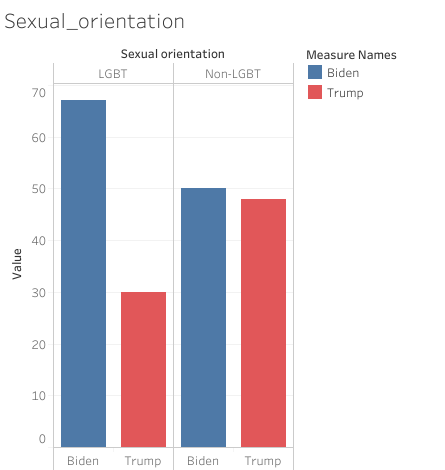
\includegraphics[width=0.55\textwidth]{figures/Sexual_orientation.png}
        \caption{Tỷ lệ ủng hộ ứng cử viên theo xu hướng giới tính}
    \end{figure}
\end{frame}


\begin{frame}{Tỷ lệ ủng hộ ứng cử viên theo số lần đi bỏ phiếu}
	\begin{figure}[h!]
        \centering
        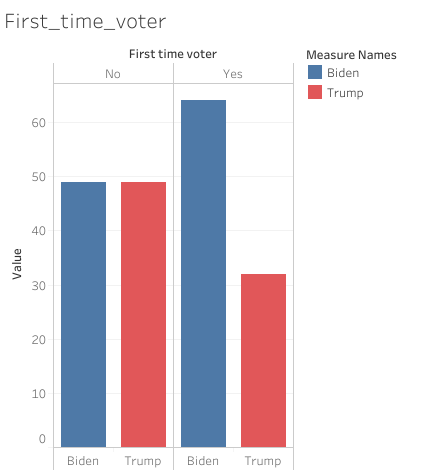
\includegraphics[height=0.65\textheight]{figures/First_time_voter.png}
        \caption{Tỷ lệ ủng hộ ứng cử viên theo số lần đi bỏ phiếu}
    \end{figure}
\end{frame}

\begin{frame}{Tỷ lệ ủng hộ ứng cử viên theo thu nhập}
	\begin{figure}[h!]
        \centering
        \includegraphics[width=0.7\textwidth]{figures/income.png}
        \caption{Tỷ lệ ủng hộ ứng cử viên theo thu nhập}
    \end{figure}
\end{frame}


\begin{frame}{Tỷ lệ ủng hộ ứng cử viên theo khu vực}
	\begin{figure}[h!]
        \centering
        \includegraphics[width=0.6\textwidth]{figures/region.png}
        \caption{Tỷ lệ ủng hộ ứng cử viên theo khu vực}
    \end{figure}
\end{frame}

\begin{frame}{Tỷ lệ ủng hộ ứng cử viên theo tình trạng tài chính}
	\begin{figure}[h!]
        \centering
        \includegraphics[width=0.6\textwidth]{figures/family_financial_situation.png}
        \caption{Tỷ lệ ủng hộ ứng cử viên theo tình trạng tài chính}
    \end{figure}
\end{frame}

\begin{frame}{Tỷ lệ ủng hộ ứng cử viên theo phục vụ quân ngũ}
	\begin{figure}[h!]
        \centering
        \includegraphics[height=0.7\textheight]{figures/Military_service.png}
        \caption{Tỷ lệ ủng hộ ứng cử viên theo phục vụ quân ngũ}
    \end{figure}
\end{frame}

\begin{frame}{Tỷ lệ ủng hộ ứng cử viên theo cách nhìn nhận các vấn đề xã hội}
	\begin{figure}[h!]
        \centering
        \includegraphics[width=0.8\textwidth]{figures/Issue_regarded_as_most_important.png}
        \caption{Tỷ lệ ủng hộ ứng cử viên theo cách nhìn nhận các vấn đề xã hội}
    \end{figure}
\end{frame}

\begin{frame}{Tỷ lệ ủng hộ ứng cử viên theo khu vực sinh sống}
	\begin{figure}[h!]
        \centering
        \includegraphics[width=0.6\textwidth]{figures/area_type.png}
        \caption{Tỷ lệ ủng hộ ứng cử viên theo khu vực sinh sống}
    \end{figure}
\end{frame}

\begin{frame}{Tỷ lệ ủng hộ ứng cử viên theo quan điểm về nạo phá thai}
	\begin{figure}[h!]
        \centering
        \includegraphics[height=0.7\textheight]{figures/abortion_should_be.png}
        \caption{Tỷ lệ ủng hộ ứng cử viên theo quan điểm về nạo phá thai}
    \end{figure}
\end{frame}

\section{Xây dựng mô hình}

\begin{frame}
	\begin{itemize}
		\item Loại mô hình thứ nhất là mô hình hồi quy dự đoán tỷ lệ phiếu bầu của ứng viên đảng Cộng hòa tại một hạt.
		\item Loại mô hình thứ hai là mô hình phân loại dự đoán liệu ứng viên đảng Cộng hòa có thắng tại hạt đó hay không.
	\end{itemize}
\end{frame}

\begin{frame}{Mô hình hồi quy}

    \begin{itemize}
        \item Mô hình đơn giản, ta chỉ tính trung bình tỷ lệ được bỏ phiếu tại tất cả các hạt.
        \item Mô hình thứ hai là sử dụng mô hình hồi quy tuyến tính.
        \item Mô hình thứ ba là mô hình XGBoost.
    \end{itemize}
\end{frame}

\begin{frame}{Mô hình phân loại}
	\begin{itemize}
        \item Logistic Regression
        \item Random Forest
        \item Decision Tree
        \item XGBoost Classification
    \end{itemize}
\end{frame}

\begin{frame}
    \begin{figure}[h!]
        \centering
        \includegraphics[height=0.85\textheight]{figures/Box_plot.png}
        \caption{Biểu diễn box plot của các đặc trưng}
    \end{figure}
\end{frame}

\subsection{Mô hình hồi quy}

\begin{frame}{Kết quả mô hình hồi quy tuyến tính}
	\begin{figure}[h!]
        \centering
        \includegraphics[height=0.75\textheight]{figures/GLM_Result.png}
        \caption{Kết quả của mô hình hồi quy tuyến tính}
    \end{figure}
\end{frame}

\begin{frame}{Độ quan trọng của các đặc trưng trong mô hình XGBoost Regression}
	\begin{figure}[h!]
        \centering
        \includegraphics[height=0.65\textheight]{figures/XGBoost_Regression_Feature_Importance.png}
        \caption{Độ quan trọng của các đặc trưng trong mô hình XGBoost Regression}
    \end{figure}
\end{frame}


\begin{frame}{Bảng kết quả dự đoán các phương pháp trong mô hình hồi quy}
	\begin{figure}[h!]
        \centering
        \includegraphics[width=0.7\textwidth]{figures/Regression_Model_Result.png}
        \caption{Bảng kết quả dự đoán các phương pháp trong mô hình hồi quy}
    \end{figure}
\end{frame}

\begin{frame}{Kết quả độ đo RMSE của các phương pháp}
	\begin{figure}[h!]
        \centering
        \includegraphics[height=0.6\textheight]{figures/Regression_Model_Result_RMSE.png}
        \caption{Kết quả độ đo RMSE của các phương pháp}
    \end{figure}
	Ta nhận thấy XGBoost có kết quả tốt hơn nhiều so với mô hình hồi quy tuyến tính.
    Mô hình hồi quy tuyến tính cho kết quả dự đoán không tốt do không giải thích được với dữ liệu.
\end{frame}

\subsection{Mô hình phân loại}

\begin{frame}{Kết quả phân loại với mô hình logistic}
	\begin{figure}[h!]
        \centering
        \includegraphics[width=0.6\textwidth]{figures/Logistic_Regression_Report.png}
        \caption{Kết quả phân loại với mô hình logistic}
    \end{figure}
\end{frame}


\begin{frame}{Độ quan trọng của các đặc trưng trong mô hình Logistic Regression}
	\begin{figure}[h!]
        \centering
        \includegraphics[width=0.7\textwidth]{figures/Logistic_Regression_Feature_Importance.png}
        \caption{Độ quan trọng của các đặc trưng trong mô hình Logistic Regression}
    \end{figure}
\end{frame}

\begin{frame}{Kết quả phân loại với mô hình Random Forest}
	\begin{figure}[h!]
        \centering
        \includegraphics[width=0.6\textwidth]{figures/Random_Forest_Feature_Report.png}
        \caption{Kết quả phân loại với mô hình Random Forest}
    \end{figure}
\end{frame}

\begin{frame}{Độ quan trọng của các đặc trưng trong mô hình Random Forest}
	\begin{figure}[h!]
        \centering
        \includegraphics[height=0.7\textheight]{figures/Random_Forest_Feature_Importance.png}
        \caption{Độ quan trọng của các đặc trưng trong mô hình Random Forest}
    \end{figure}
\end{frame}

\begin{frame}
	\begin{figure}[h!]
        \centering
        \includegraphics[width=0.6\textwidth]{figures/Decision_Tree_Report.png}
        \caption{Kết quả phân loại với mô hình Decision Tree}
    \end{figure}
\end{frame}

\begin{frame}{Độ quan trọng của các đặc trưng trong mô hình Decision Tree}
	\begin{figure}[h!]
        \centering
        \includegraphics[height=0.7\textheight]{figures/Decision_Tree_Feature_Importance.png}
        \caption{Độ quan trọng của các đặc trưng trong mô hình Decision Tree}
    \end{figure}
\end{frame}

\begin{frame}{Kết quả phân loại với mô hình XGBoost Classification}
	\begin{figure}[h!]
        \centering
        \includegraphics[width=0.6\textwidth]{figures/XGBoost_Classifier_Report.png}
        \caption{Kết quả phân loại với mô hình XGBoost Classification}
    \end{figure}
\end{frame}

\begin{frame}{Độ quan trọng của các đặc trưng trong mô hình XGBoost Classification}
	\begin{figure}[h!]
        \centering
        \includegraphics[height=0.7\textheight]{figures/XGBoost_Regression_Feature_Importance.png}
        \caption{Độ quan trọng của các đặc trưng trong mô hình XGBoost Classification}
    \end{figure}
\end{frame}

\begin{frame}{Tỷ lệ người da trắng theo từng hạt}
	\begin{figure}[h!]
        \centering
        \includegraphics[width=0.9\textwidth]{figures/County_Percentage_White_People.png}
        \caption{Tỷ lệ người da trắng theo từng hạt}
    \end{figure}
\end{frame}

\section{Kết luận}

\begin{frame}{Kết luận}
	\begin{itemize}
        \item Đa số những người da trắng ủng hộ đảng Cộng hòa và ngược lại các chủng tộc khác đa số ủng hộ đảng Dân chủ.
        \item Những người ủng hộ đảng Cộng hòa thường có xu hướng bảo thủ, bảo vệ giá trị truyền thống và ngược lại những người có xu hướng cởi mở, tiến bộ thường hay ủng hộ đảng Dân chủ.
        \item Nhóm có tầng lớp dân trí cao thường hay ủng hộ đảng Dân chủ.
        \item Nam giới (da trắng) có xu hướng ủng hộ đảng Cộng hòa.
        \item Cư dân tại nông thôn, vùng núi có xu hướng ủng hộ Đảng Cộng hòa và ngược lại, cư dân tại thành thị, ngoại ô có xu hướng ủng hộ Đảng Dân chủ.
        \item Đảng Cộng hòa thắng tại đa số diện tích nước Mỹ nhưng chủ yếu là các vùng ít dân cư và hay thua tại các vùng đông dân cư.
    \end{itemize}
\end{frame}

\section{Tài liệu tham khảo}
\begin{frame}[allowframebreaks]{Tài liệu tham khảo}
    \printbibliography
\end{frame}

\end{document}